\chapter{Laboratorio 4}

Il primo circuito analizzato è il multivibratore monostabile (\Fig\ref{fig:circuito_1}). Tale circuito presenta uno stato stabile, in cui rimane fino a che un impulso esterno di comando lo porta in un secondo stato, in cui il circuito rimane per un tempo predefinito per poi tornare spontaneamente nello stato stabile, in attesa di un successivo impulso.
\begin{figure}[h]
	\centering
	\begin{minipage}{.45\textwidth}
		\scalebox{.62}{
			\begin{circuitikz}
				\draw (2,6) node[op amp, anchor=-](oa){\texttt{TL071}};
				\draw (oa.-) -- ++(-2, 0) coordinate (D) -- ++(-2,0) to[C=$C$] ++(0,-1.5) node[ground]{};
				\draw (D) to[D=$D$] ++(0,-1.5) node[ground]{};
				\draw (oa.up) -- ++(0, 0.3) node[vcc]{$V_{DD}$};
				\draw (oa.down) -- ++(0,-0.3) node[vee]{$V_{SS}$};
				\draw (oa.out) -- ++(1,0) coordinate(loop);
				\draw (loop) -- ++(0,-2.3) coordinate(R2) to[R=$R_2$] ++(-3.39,0) coordinate(rg) (R2-|oa.+) -- (oa.+);
				\draw (oa.-) -- ++(0,1.7) to[R=$R_3$]++(3.39,0) coordinate(Rf) (Rf-|loop) -- (loop);
				\draw (oa.+) to[short, -o] ++(0,0) ++(-.1,0) node[left]{$v_+$};
				\draw (oa.-) to[short, -o] ++(0,0) ++(0,-.1) node[below]{$v_-$};
				\draw (rg) -- ++(-1,0) coordinate(r1) to[R=$R_1$] ++(0,-2) node[ground]{};
				\draw (r1) to[D=$D_T$] ++(-2.5,0) coordinate(vt) to[C=$C_T$] ++(-3,0) coordinate(vin);
				\draw (vt) to[R=$R_T$] ++(0,-2) node[ground]{};
				\draw (vt) to[short, -o] ++(0,0) node[above]{$v_t$};
				\draw (loop) to[short, -o] ++(0,0) ++(.1,0) node[right]{$v_{out}$};
				\draw (vin) to[sqV=$v_{in}$] ++(0,-2) node[ground]{};
				\draw[thick] (-5.5,0) rectangle (6.5,8.5);
			\end{circuitikz} 
		}
	\end{minipage}\qquad
	\begin{minipage}{.45\textwidth}
		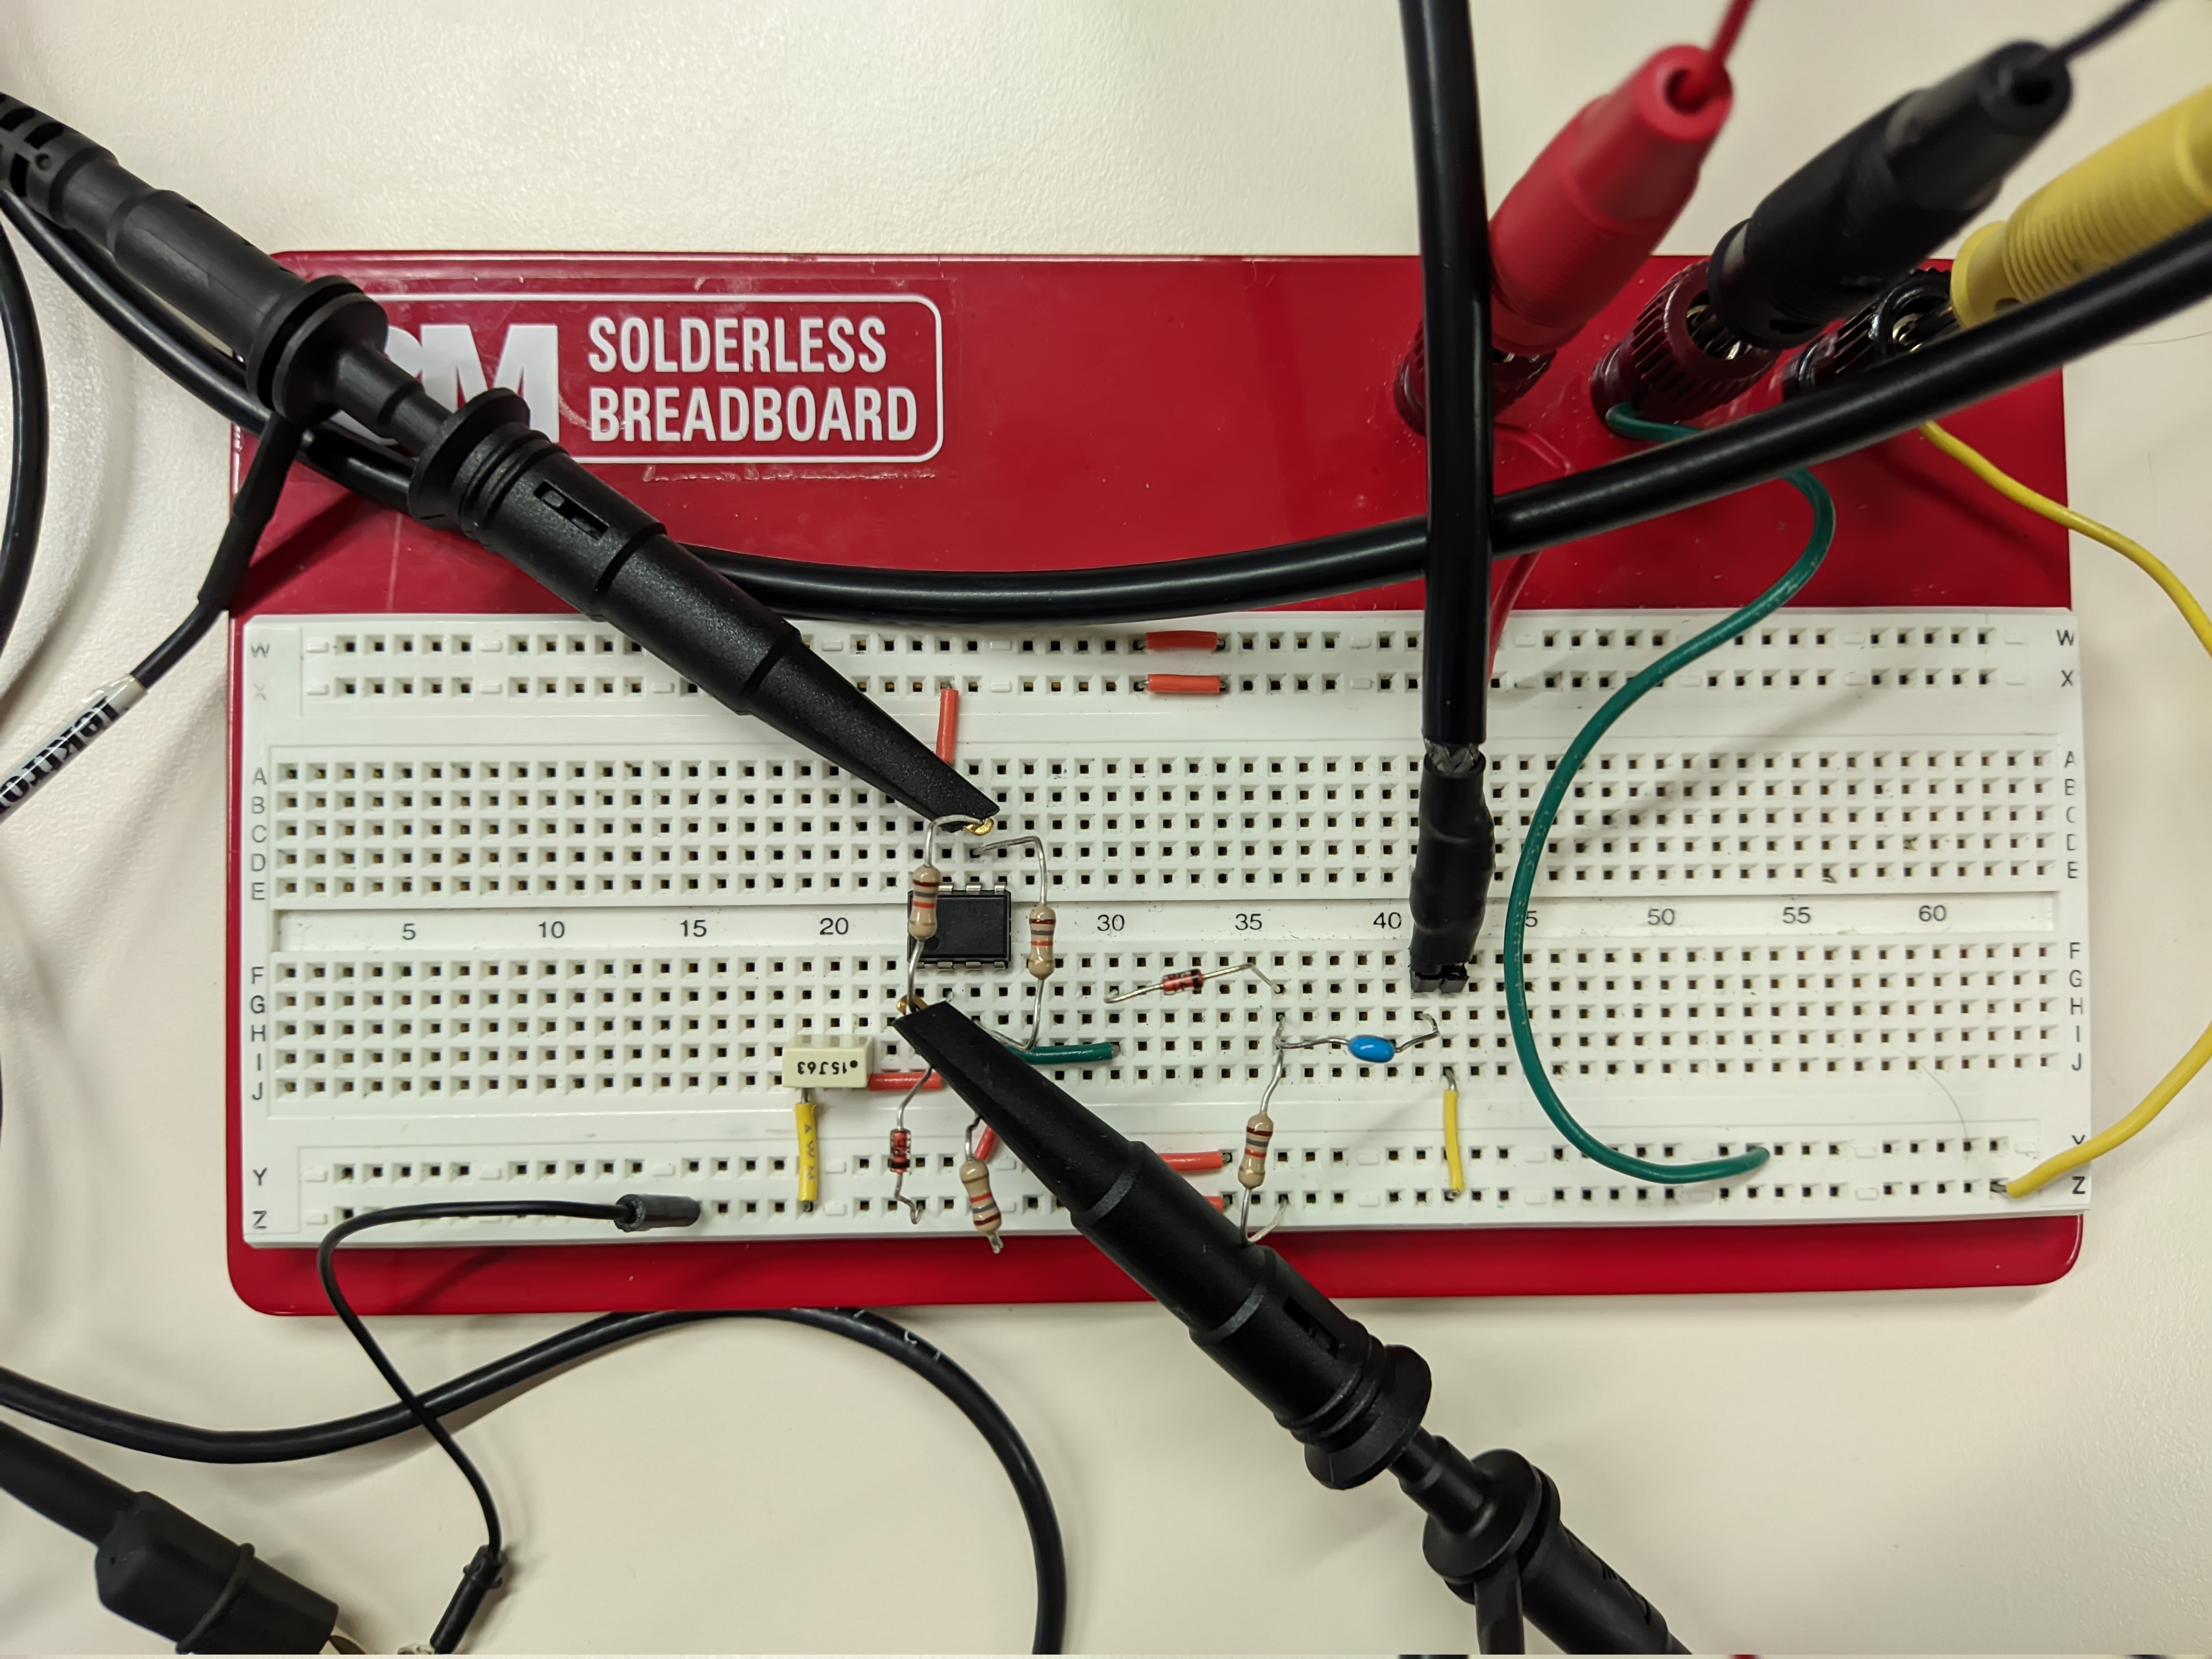
\includegraphics[width=\linewidth]{./ImageFiles/Laboratorio 4/CIR11.jpg}
	\end{minipage}
	\caption{Schema circuitale del multivibratore monostabile e foto del circuito realizzato.}
	\label{fig:circuito_1}
\end{figure}
Per realizzare il circuito, si parte dal generatore d'onda quadra visto nella precedente esperienza di laboratorio. Inserendo un diodo $D$ in parallelo alla capacità $C$ si ottiene uno stato stabile. Supponiamo che inizialmente la tensione di uscita sia pari a V\sub{DD} e che la capacità sia scarica. Allora, la capacità si carica attraverso la resistenza R\sub{3} fino a quando la tensione ai suoi capi raggiunge circa \SI{0.7}{\volt} (tensione di polarizzazione del diodo $D$). A questo punto, il processo di carica si interrompe perché il diodo si accende e si comporta come un cortocircuito. Quindi la corrente scorrerà solo attraverso il diodo $D$ verso massa. Quindi l'uscita rimane stabile alla tensione V\sub{DD}.

\noindent
Affinché il circuito commuti dallo stato stabile $v_{out}=V_{DD}$ allo stato quasi stabile $v_{out}=V_{SS}$ è necessario che la tensione dell'ingresso non invertente scenda al di sotto della tensione dell'ingresso invertente. Questo viene reso possibile applicando sul morsetto non invertente un impulso negativo di tensione. Per fare ciò si inserisce un circuito derivatore composto da una capacità $C_T$ ed una resistenza $R_T$. Tale circuito ha il compito di generare, a partire da un segnale rettangolare $v_{in}$, un impulso positivo ed uno negativo. Questi \textit{spike} di tensione sono generati sui fronti di salita e discesa dell'onda quadra in ingresso. Il diodo $D_T$ permette di non trasmettere gli impulsi positivi al nodo V\super{+} (il diodo infatti si spegne) ma lascia passare inalterati gli impulsi negativi.
Questo impulso negativo generato porterà per un breve istante la tensione $v_+$ al di sotto della tensione presente ai capi del condensatore (che è pari alla tensione di polarizzazione del diodo) forzando la commutazione dell'uscita a $v_{out}=V_{SS}$. A questo punto, il condensatore si scarica fino a raggiungere la tensione di soglia $V_H^+=\frac{1}{2}V_{SS}$ dove l'uscita commuta portandosi a $v_{out}=V_{DD}$. Il condensatore ricomincia così il ciclo di carica ma termina una volta raggiunta la tensione di polarizzazione del diodo (che è minore della nuova tensione di soglia V\sub{H}\super{+}) . Il circuito entra di nuovo in uno stato stabile in attesa che sul morsetto non invertente venga generato un altro impulso negativo. Il tempo per cui $v_{out}=V_{SS}$ dipende dalla capacità $C$ e dalla resistenza $R3$.

\noindent
I valori utilizzati nel circuito sono indicati nella tabella \ref{tab:valori_componenti_1}. L'amplificatore scelto è il \textbf{TL071} ed è stato alimentato con una tensione duale di $\pm$\SI{10}{\volt}.

\def\arraystretch{1.3}
\begin{table}[h!]
	\centering
	\begin{tabular}{|c|c|c|}
		\hline
		Componente	& Valore Nominale & Valore Misurato \\ \hline
		R1 &\SI{18}{\kilo\ohm} & \SI{17,96}{\kilo\ohm} \\ \hline
		R2 &\SI{18}{\kilo\ohm} & \SI{17,79}{\kilo\ohm} \\ \hline
		R3 & \SI{18}{\kilo\ohm} & \SI{18}{\kilo\ohm} \\ \hline
		R\sub{T} & \SI{18}{\kilo\ohm} & \SI{17,83}{\kilo\ohm} \\ \hline
		D\sub{T} & $\simeq$\SI{0.7}{\volt} & \SI{609}{\milli\volt} \\ \hline
		D1 & $\simeq$\SI{0.7}{\volt} & \SI{607}{\milli\volt} \\ \hline
		C & \SI{150}{\nano\farad} & Non misurato \\ \hline
	\end{tabular}
	\caption{Valori nominali e misurati dei componenti utilizzati nel circuito.}
	\label{tab:valori_componenti_1}
\end{table}

\noindent
Per generare gli impulsi di tensione, si è utilizzato un segnale in ingresso ad onda quadra con \textit{duty-cicle} pari al 20\%, frequenza di \SI{100}{\hertz} e ampiezza picco-picco pari a \SI{5}{\volt}\todo{Inserire valori corretti}. In figura \ref{fig:picchi_ingresso} si vedono i picchi generati dal derivatore. 

\begin{figure}[h!]
	\centering
	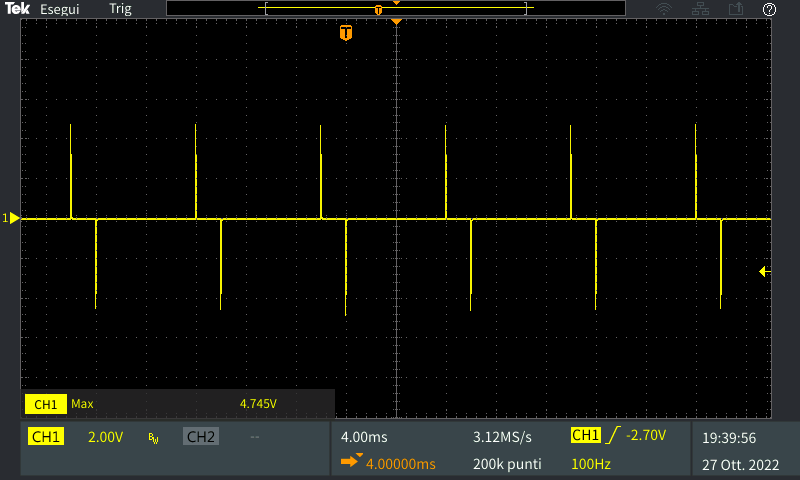
\includegraphics[width=\linewidth]{./ImageFiles/Laboratorio 4/TEK00002.PNG}
	\caption{Misure del segnale $v_{t}$ (linea gialla). Questi picchi sono generati dal circuito derivatore con in ingresso un'onda quadra con \textit{duty-cicle} del 20\%, frequenza di \SI{100}{\hertz} e ampiezza picco-picco pari a \SI{10}{\volt}.}
	\label{fig:picchi_ingresso}
\end{figure}

\noindent
In figura \ref{fig:segnale_uscita} sono invece mostrati gli andamenti di $v_{-}$ e $v_{out}$. È interessante notare che i valori di saturazione dell'amplificatore operazionale, e quindi i valori tra cui commuta $v_{out}$, sono minori delle tensioni di alimentazione $V_{DD}$ e $V_{SS}$.
\begin{figure}[h!]
	\centering
	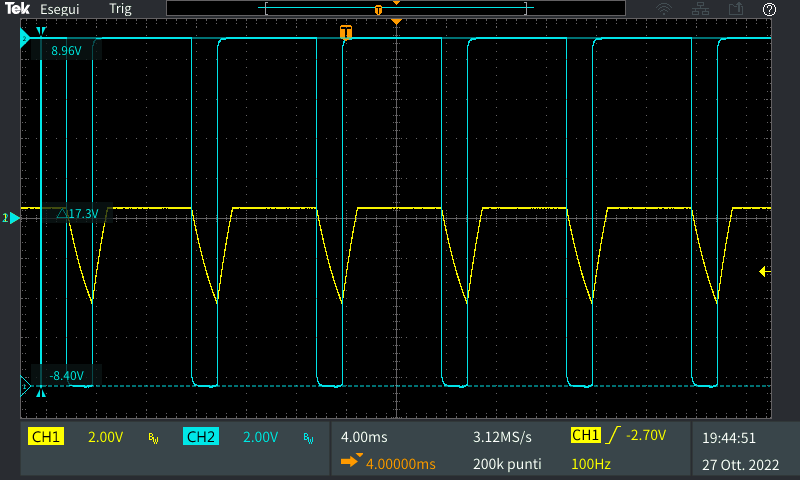
\includegraphics[width=\linewidth]{./ImageFiles/Laboratorio 4/TEK00008.PNG}
	\caption{Misure del segnale $v_{-}$ (linea gialla) e del segnale $v_{out}$ (linea azzurra).}
	\label{fig:segnale_uscita}
\end{figure}

\noindent
\`E stato inoltre possibile misurare il tempo in cui l'uscita rimane alla tensione V\sub{SS} (che indichiamo con T\sub{A}). Infatti, esso dipende dalla costate di tempo di carica e scarica $\tau=R_3C$ e dai valori delle resistenze R\sub{1} e R\sub{2}. Infatti, indicando con t\sub{1} l'istante in cui la tensione la nodo V\super{-} raggiunge la tensione soglia V\super{L}\super{+} e considerando t\sub{0} l'istante in cui viene applicato l'impulso negativo si ha che
\begin{equation}
	V^-(t_1)=V_{SS}+(\SI{0.7}{\volt}-V_{SS})e^{\frac{-t_1}{\tau}}=V_L^+
\end{equation}
e quindi, considerando $|V_{SS}|\gg\SI{0.7}{\volt}$ si ottiene
\begin{equation}
	t_A=\tau\ln\left(1+\frac{R_2}{R_1}\right).
	\label{eq:ta}
\end{equation}
Attraverso i cursori forniti dall'oscilloscopio si ricava che il tempo t\sub{A} è pari a \SI{1.78}{\milli\second} (\Fig\ref{fig:calcolo_ta}), mentre il valore teorico dato dall'equazione \ref{eq:ta} è di \SI{1.86}{\milli\second}.

\begin{figure}[h!]
	\centering
	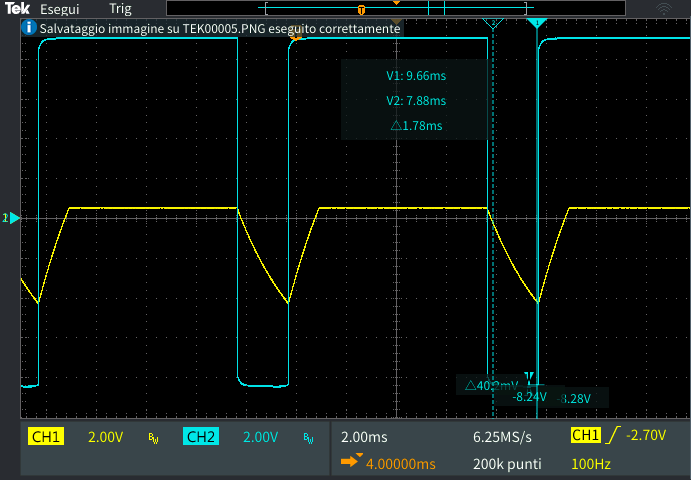
\includegraphics[width=\linewidth]{./ImageFiles/Laboratorio 4/TEK00006.PNG}
	\caption{Misure del segnale $v_{-}$ (linea gialla) e del segnale $v_{out}$ (linea azzurra).}
	\label{fig:calcolo_ta}
\end{figure}

\newpage
Il secondo circuito visto a lezione è una variante del circuito precedente implementata tramite un integrato 555 al posto di un amplificatore operazionale (Fig \ref{fig:circuito_2}).
\begin{figure}[h!]
	\centering
	\begin{minipage}{.45\textwidth}
		\scalebox{.47}{
			\begin{circuitikz}
				%Main dip package
				\draw (0,0) node[dipchip,num pins=8, hide numbers, external pins width=0.1, scale=3, external pad fraction=6](C){NE555};
				%Pin names
				\node [right] at (C.bpin 1) {GND};
				\node [right] at (C.bpin 2) {TRIG};
				\node [right] at (C.bpin 3) {OUT};
				\node [right] at (C.bpin 4) {RST};
				\node [left] at (C.bpin 5) {CV};
				\node [left] at (C.bpin 6) {THRS};
				\node [left] at (C.bpin 7) {DISCH};
				\node [left] at (C.bpin 8) {$V_{CC}$};
				%Connections
				\draw (C.pin 1) -- ++(-4,0) -- ++(0,-6) node[ground]{};
				\draw (C.pin 8) -- ++(2,0) coordinate(vcc) -- ++(0,1.35) node[vcc]{$V_{CC}$};
				\draw (C.pin 7) -- ++(2,0) coordinate(dsc) to[R=$R$] (vcc);
				\draw (C.pin 6) -- ++(2,0) coordinate(trs) -- (dsc);
				\draw (trs) -- ++(2,0) to[C=$C$] ++(0,-2.68) node[ground]{};
				\draw (C.pin 5) -- ++(2,0) to[C=$C_2$] ++(0,-1) node[ground]{};
				\draw (C.pin 4) -- ++(-1.5,0) -- ++(0,3) to[crossing] ++(0,.72) to[crossing] ++ (0,2.64) node[vcc]{$V_{CC}$};
				\draw (C.pin 3) to[short, -o] ++(-1,0) ++(0,.1) node[above]{$v_{out}$};
				\draw (C.pin 2) -- ++(-3,0) coordinate(vin);
				\draw (vin) to[sqV=$v_{in}$] ++(0,-2) node[ground]{};
				\draw[thick] (-7.5,-5.3) rectangle (8,5.9);
			\end{circuitikz}
		}
\end{minipage}\qquad
\begin{minipage}{.45\textwidth}
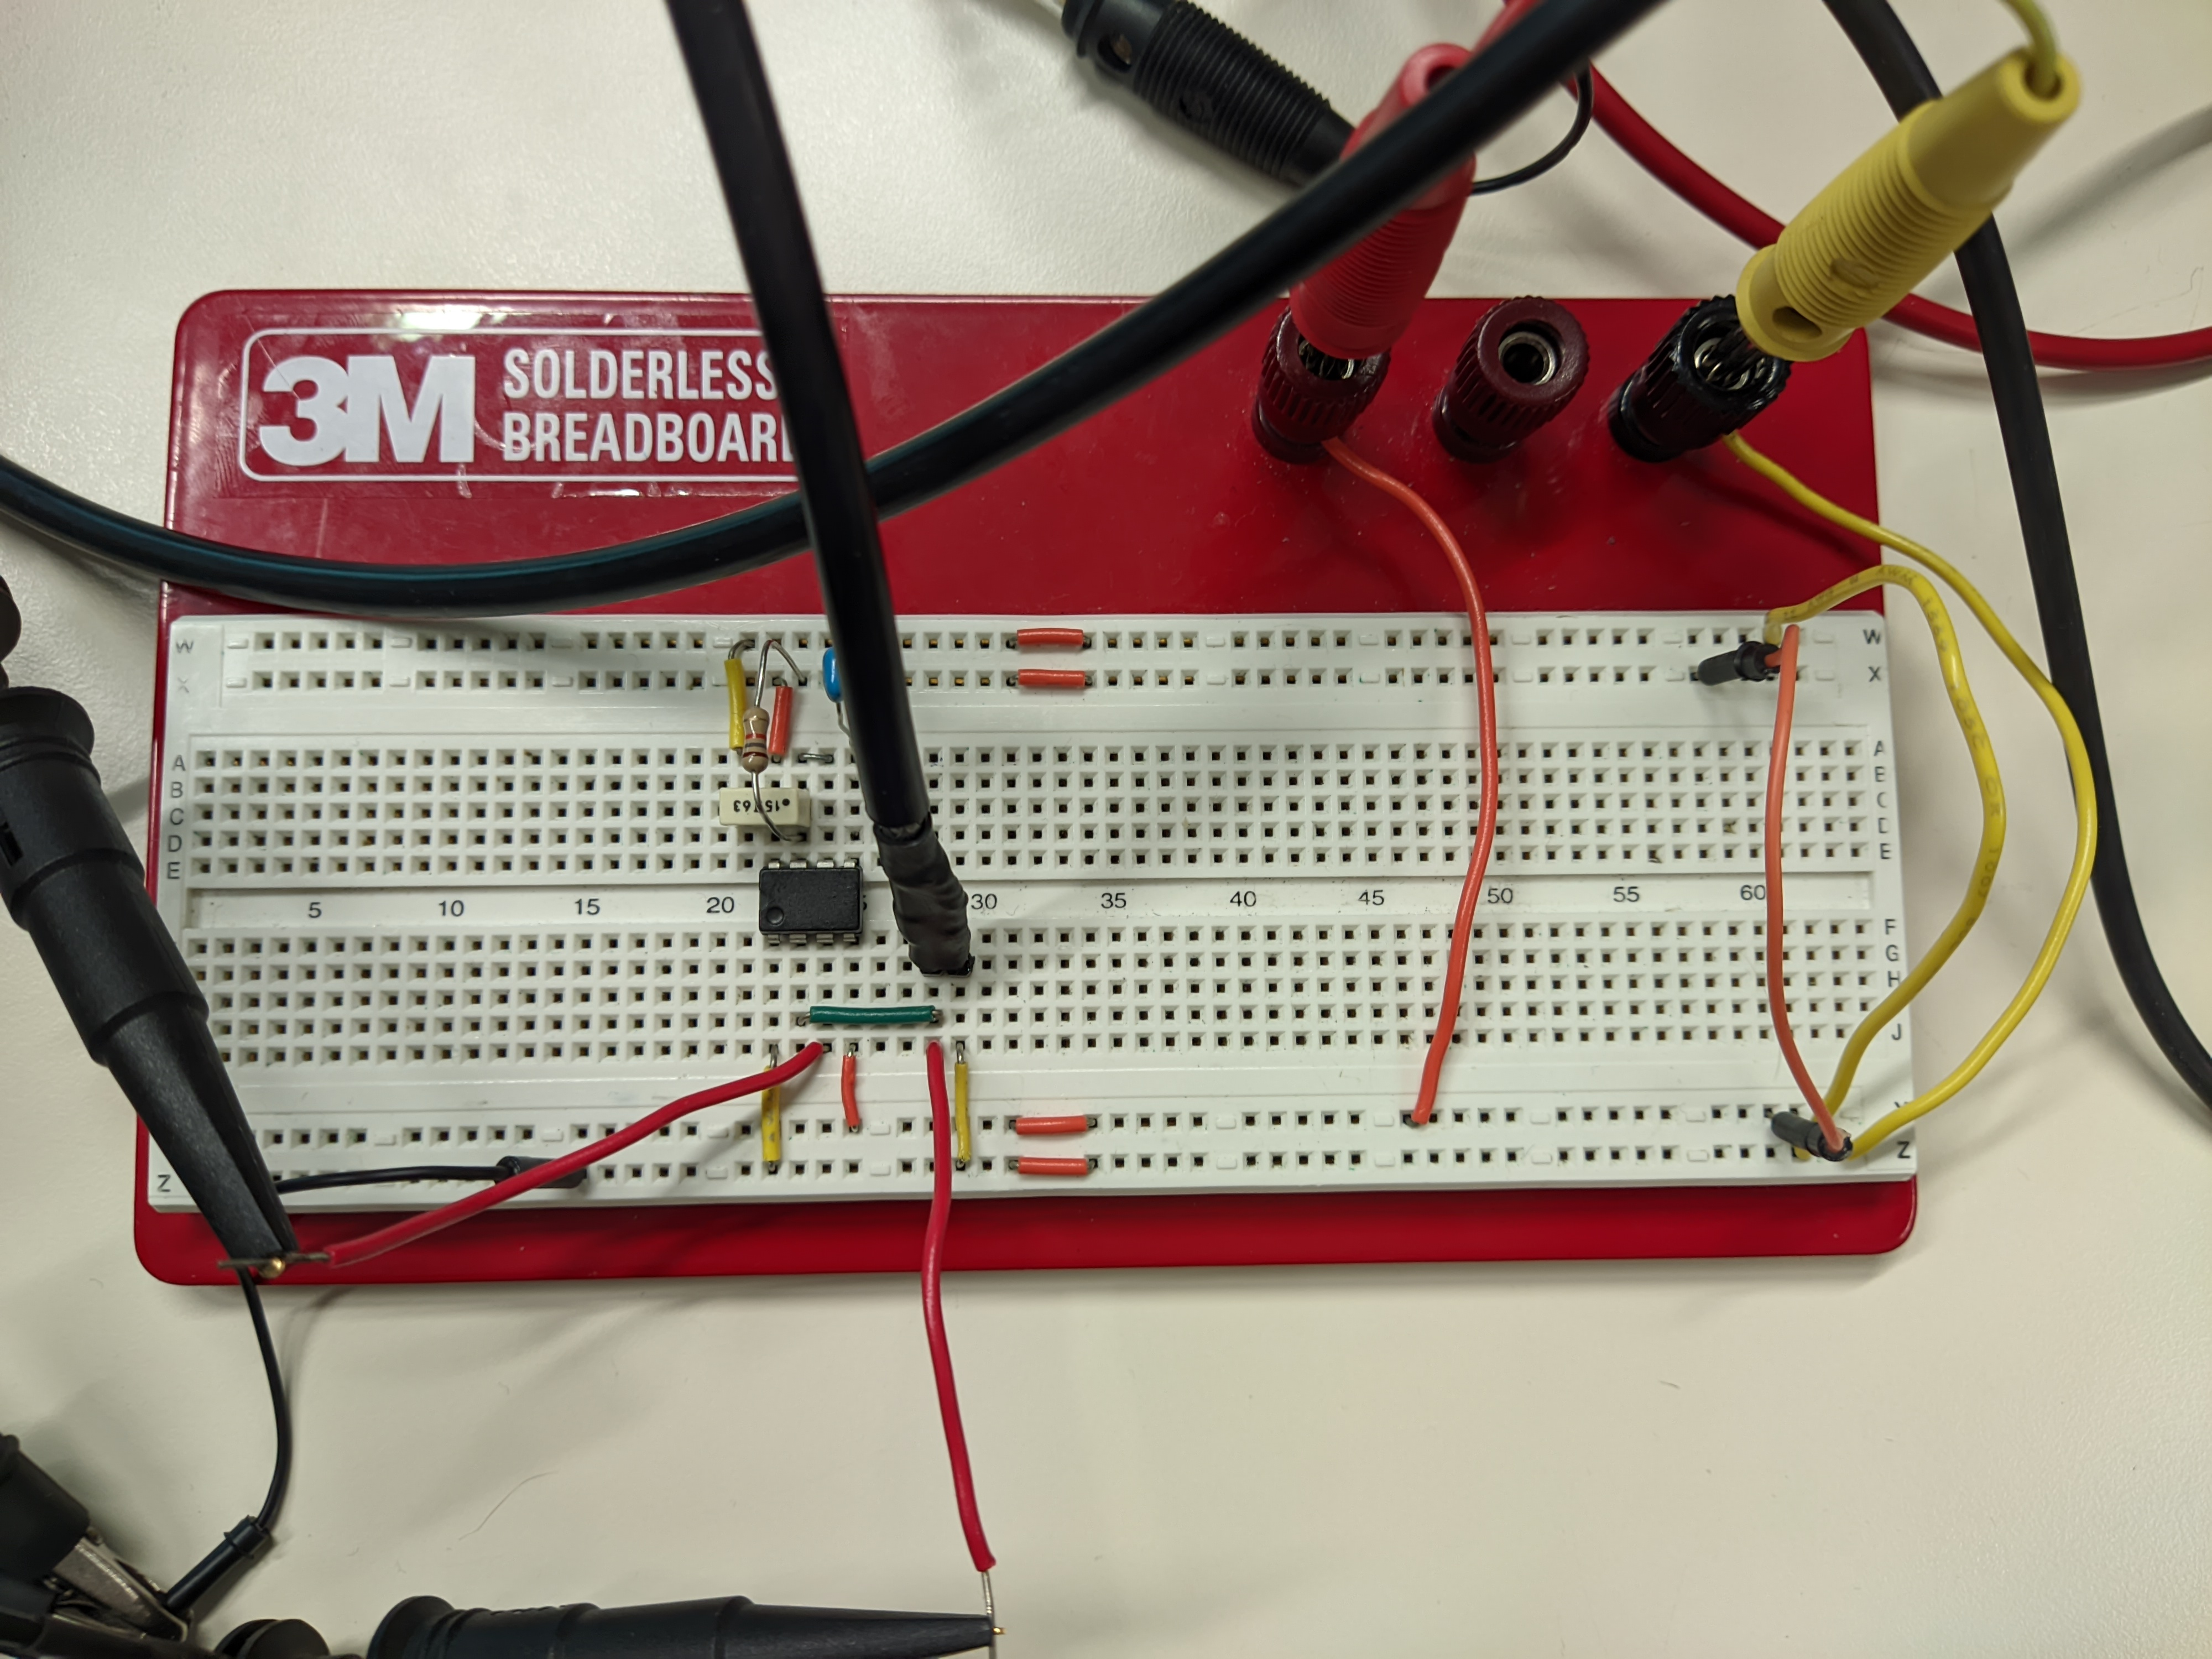
\includegraphics[width=\linewidth]{./ImageFiles/Laboratorio 4/CIR21.jpg}
\end{minipage}
\caption{Schema circuitale del 555 monostabile e foto del circuito realizzato.}
\label{fig:circuito_2}
\end{figure}
\todo{Qualcuno si è scritto/ricorda il nome specifico dell'integrato?}
\begin{figure}[h!]
	\centering
	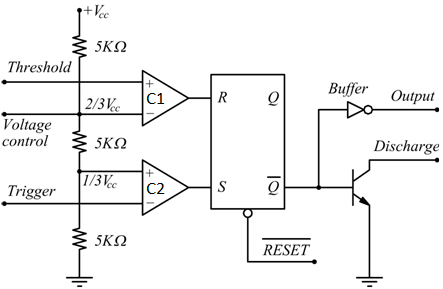
\includegraphics[width=\linewidth]{./ImageFiles/Laboratorio 4/555internals.jpg}
	\caption{Struttura interna di un circuito integrato 555}
	\label{fig:555_internals}
\end{figure}

\noindent
Come si può vedere dall'immagine \ref{fig:555_internals}, il 555 è composto da due comparatori collegati ad un flip flop alle loro corrispondenti uscite. Il comparatore in alto ha $\frac{2}{3}V_{CC}$ della tensione di alimentazione fornita in ingresso all'integrato. Tensioni maggiori provocano la commutazione al livello logico alto. Questa è anche collegata ad un piedino esterno in modo da permettere di collegare una capacità aggiuntiva per migliorarne la stabilità. Il compratore in basso invece ha collegato al morsetto non invertente $\frac{1}{3}V_{CC}$ della tensione applicata all'integrato. Per poterlo far commutare ad uno stato alto quindi la tensione applicata al trigger deve essere inferiore del riferimento.

Il flip flop ha due uscite, la prima è l'uscita del flip flop; la seconda è l'uscita negata.
Le possibili combinazioni dell'uscita del flip flop set-reset sono indicate nella tabella \ref{tab:flip_flop_states}:

\def\arraystretch{1.3}
\begin{table}[h!]
	\centering
	\begin{tabular}{|c|c|c|}
		\hline
		Stato SET	& Stato RESET & Uscita \\ \hline
		Basso & Basso & Stato precedente  \\ \hline
		Alto & Basso & Alto\\ \hline
		Basso & Alto & Basso\\ \hline
		Alto & Alto & Stato proibito \\ \hline
	\end{tabular}
	\caption{Possibili stati di un flip flop SR}
	\label{tab:flip_flop_states}
\end{table}

Il 555 ha quindi collegato all'uscita negata del flip flop il controllo di un interruttore, dove su un lato è collegato a massa e l'altro lato è collegato ad un piedino chiamato discharge.

\noindent
Questo integrato inoltre, a differenza degli operazionali visti precedentemente, non utilizza due tensioni e un riferimento a massa, ma soltanto una tensione positiva e il riferimento a massa. Nel nostro caso specifico l'integrato è stato alimentato con una tensione positiva di \SI{10}{\volt}.

\noindent
Quando l'uscita del generatore di segnale collegato tra il trigger e la massa del circuito 555 rimane a $V_{CC}$, che è maggiore della tensione di soglia di $\frac{1}{3}V_{CC}$.

\noindent
Se ipotizzo che il suo stato iniziale non sia settato, il flip flop mantiene lo stato basso in uscita, e di conseguenza uscita negata risulta alta. Ciò mantiene chiuso l'interruttore che collega a massa il discharge, treshhold e la capacità, mantenendo quindi il circuito in questo stato fino a quando il trigger non commuta ad uno stato basso.

\noindent
Quando il generatore di segnale cambia stato, il morsetto del secondo comparatore risulta più negativo della tensione di soglia del comparatore. Questo lo porta ad un cambio di stato (instabile) e il flip flop viene settato portando l'uscita ad uno stato alto. Ciò causa l'apertura dell'interruttore scollegando il pin DISCH da massa, lasciandolo flottante.
La capacità può iniziare a caricarsi lentamente tramite la resistenza $R$ messa tra il condensatore e $V_{CC}$. La capacità continuerebbe a caricarsi fino a raggiungere una tensione pari a $V_{CC}$, ma uno dei suoi capi è collegato al primo comparatore, che è collegato ad una tensione di riferimento di $\frac{2}{3}V_{CC}$ sul suo morsetto negativo. 

\noindent
Quando quindi il morsetto positivo supera questa soglia, il comparatore imposterà la sua uscita ad un livello alto, resettando quindi il flip flop. Ciò riporterà la sua uscita ad un livello basso, l'interruttore verrà nuovamente chiuso e la capacità verrà cortocircuitata, forzandone la scarica verso massa. Ciò riporta il circuito allo stato iniziale.

\noindent
Il periodo di carica e scarica varia in base ai valori di $R$ e di $C$, seguendo la relazione
\[v_C = V_{CC}\cdot\left(1-e^{-\frac{t}{RC}}\right)\]
La carica della capacità termina quando $v_C = \frac{2}{3}V_{CC}$, quindi
\[\frac{2}{3}V_{CC} = V_{CC}\cdot\left(1-e^{-\frac{T}{RC}}\right)\]
\[T=-RC\ln\left(\frac{1}{3}\right)\approx1.1RC\]

Per caratterizzare questo circuito abbiamo quindi provato a sostituire valori di $R$ e di $C$ per verificare la validità dell'equazione scritta sopra. Nella tabella \ref{tab:valori_componenti_2} sono indicati i valori che abbiamo scelto.

\def\arraystretch{1.3}
\begin{table}[h]
	\centering
	\begin{tabular}{|c|c|c|}
		\hline
		Componente	& Valore Nominale & Valore Misurato \\ \hline
		R1 &\SI{10}{\kilo\ohm} & \SI{10,96}{\kilo\ohm} \\ \hline
		R2 &\SI{18}{\kilo\ohm} & \SI{18,02}{\kilo\ohm} \\ \hline
		R3 & \SI{12}{\kilo\ohm} & \SI{11,96}{\kilo\ohm} \\ \hline
		R4 & ? & ? \\ \hline
		C1 & \SI{150}{\nano\farad} & Non misurato \\ \hline
		C2 & \SI{330}{\nano\farad} & Non misurato \\ \hline
	\end{tabular}
	\caption{Valori nominali e misurati dei componenti utilizzati nel circuito.}
	\label{tab:valori_componenti_2}
\end{table}
\todo{Completare l'ultimo valore di R usato}
Il segnale in ingresso utilizzato è un'onda quadra con \textit{duty-cicle} pari al 80\%, frequenza di \SI{100}{\hertz} e ampiezza picco-picco pari a \SI{10}{\volt}, con un offset di \SI{5}{\volt}.
\todo{Immagini e grafico di matlab risultante da aggiungere}
